\chapter{Technical Design}
\label{chap:technical}

This chapter in the thesis would have the technical design of the project.  It would contain the design details for the architecture of the solution, program flow, and the details of the components.

\section{Architectures in Unity(Introduction, discusses the component based nature of Unity)}
\subsection{Basic overview}
Developing in Unity, or any existing game engine, the engine will heavily influence the basic architecture of the solution. Therefore, a basic understanding of the Unity engine can give a better understanding of the architecture in this solution.
Every object in the game will be a GameObject. A GameObject is a container that contains components, and where you add scripts with custom behaviour.

    - Component based (different thinking to OOP)

\subsection{Networking overview}
    - Basic overview of the unity networking UNET (NetworkBehaviours)
    - Commands etc.
    - SyncVars

\section{Lobby/Main Menu}
    - Using NetworkManager / MainMenuUI for it's functionality.

\section{Ingame scene setup (Game managers and what not)}
\subsection{Ingame UI}

\section{Player architecture}

\subsection{NetworkPlayer}
    - Not destroyed on load (handles player representation in both lobby and in-game)
\paragraph{LobbyPlayer}
    - Representation in lobby
\paragraph{Player}
    - Representation in game
    
\subsection{Input}
    - PlayerInput specifics
\subsection{Field of View}
    - FieldOfView specifics
\subsection{Health and currency}
    - Health and currency specifics
    
    - Currency component is fairly simple. 
        - Uses a SyncVarHook for its currency value. 
            - SyncVarHook called whenever the server changes the currency value. 
            - Checks the difference between the new and old amount. 
            - Updates the currency value and tells the UI to update.
            - Also tells the UI to play an animation showing the difference in currency that was gained/lost.
        - Has a command for adding currency, can also be used for removing currency. 
\subsection{Player Status}
    - Specifics about player status. How it handles modifiers
\subsection{Docking}
    - Specifics on how docking works. How it is central to networking in dockit league and so on. 

\section{Modifiers architecture}
\subsection{Using scriptable objects for modifier data}

\section{Game modes}

\section{Docking Kit architecture}
\subsection{Connectivity between Ability, Docking and Docking Kit}
\subsection{Ability architecture, use of interfaces}

\section{Docking Kits}
\label{sec:dockingKits}
\subsection{Bomber Kit}
\subsection{Boomerang Kit}
The boomerang kit is a high speed, high damage kit with low health. The kit's abilities are primarily focused on augmenting the boomerangs that the player can throw. The boomerang itself has a small field of view circle around itself which allows the player to still see the boomerang if it has been thrown across a wall or other areas where vision is limited. 

\begin{figure}[tbph]  %t top, b bottom, p page | you can also use h to try to get the figure to appear at the current location
  \centering
  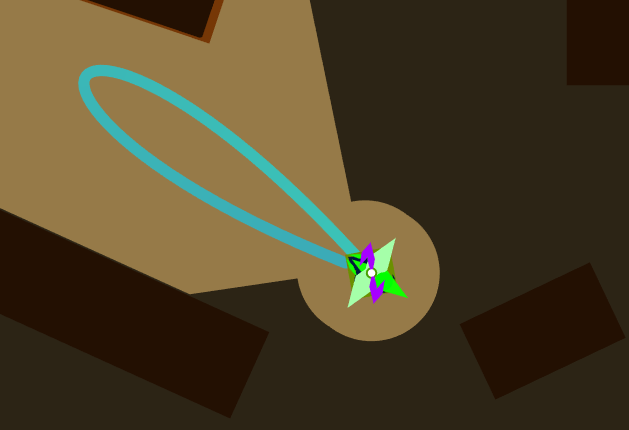
\includegraphics[width=.75\textwidth]{images/boomerangKitLineRenderer}
  \caption[Approximate travel path of the boomerang]{A screenshot from the game showing the approximate travel path of the boomerang when the ability button is held}
  \label{fig:boomerangLineRenderer}
\end{figure}

The primary ability of the boomerang kit is the boomerang throw. It uses cubic bezier curves to construct and display the approximate path that the boomerang will travel using a LineRenderer component. Figure~\ref{fig:boomerangLineRenderer} shows how the approximate path looks like for the local player using the kit. 
The bezier curvers are also used for interpolating the position of the boomerang as it is thrown by the player. The interpolation itself is handled using a timer variable that gets updated with Time.deltaTime per update loop. The timer variable is then used as input into an evaluation function used for controlling the speed of the animation and returns a smoothed version of its input. This output is then used as the input time for the bezier curve's interpolation. A more in-depth look at the interpolation of the boomerang throw can be found in section~\ref{sec:boomerangCurve}. 
    
There are also two additional boomerangs that are activated with the final ability in the kit. These have their own bezier curve control points and LineRenderers.
In order to perform the same operations on all boomerangs we have a array of structs containing the bezier control points and the stored positions of each boomerang. This allows us to modify the positions of all the bezier control points directly in the editor which makes it easy to control the shape of the curves.  

The second ability in the kit applies a root modifier to any enemy players within a certain range of the boomerang at the time of activation. It displays a range indicator for the local player whenever the ability is off cooldown making it easier to time the activation of the ability. Activating the ability will play a short ability animation around the boomerang on all clients and enables the collider component that checks for enemy players. The collider stays active for 0.5 seconds to make it a bit easier for the player using the ability to hit others as the boomerang moves at a fairly high speed. 
    
The next ability in the kit is a fairly simple ability that revolves around using a self applied modifier to control the state of its effects. Using the ability takes the field of view component of the boomerangs and quickly interpolates the radius of these to a higher value, giving the player a large circle of vision for a short duration. The additional vision is only something the local player can see while other players will see a circle indicator around the boomerang that showcases the new vision range. Once the duration of the modifier runs out the vision range quickly interpolates back to its default. 

The final ability of the boomerang kit is another self applied modifier that lasts for a few seconds and makes the next boomerang throw contain three boomerangs instead of one. This is the key ability of the kit that allows for a truly massive damage output given that the player is able to hit with all of the boomerangs. The self applied modifier is removed prematurely once a boomerang throw is made, but can also wear of naturally if the player avoids throwing any boomerangs during its duration. 

The additional boomerangs granted from this ability are also affected by the root and vision abilities, albeit with a lesser range. The boomerang throw script handles the interpolation of the two additional boomerangs while the script for this ability primarily manages the state of the buff. This includes self applying the modifier buff, managing the state of any extra visual elements and playing animations. 
    

\subsection{Brawler Kit}
The brawler kit is slow moving melee oriented kit, but has high health and multiple tools for dealing with enemies who fight at range. 

The first ability is a short cooldown slash with the brawler kit's axe. We are using OnTriggerStay instead of OnTriggerEnter as the collision callback for this ability. This is due to the fact that the animation for the slash is very quick and only lasts a few frames at its start position. Using OnTriggerEnter in this case would make the callback frequency too low at the start of the animation, essentially making it impossible to hit players nearby the start position of the axe. This happened because the first few frames would only trigger collision callbacks for the player's own overlapping collider instead of others. 
This issue is alleviated by using OnTriggerStay instead with a stored list of hit players. The list is reset after each swing and makes sure that any damage is only applied to each player once. 

The second ability in the kit is a self applied modifier that lasts for a certain duration, making the next axe slash deal increased damage and heal a certain percentage of the damage done. It works in a similar fashion to the final ability of the boomerang kit. The self applied modifier can wear of naturally or be removed after colliding with another player. Having the modifier active also changes the visuals of the axe to show that the ability has been used. 

The third ability is a self applied modifier that reflects the velocity of any projectiles that hits the player while active. This is handled using C\# interfaces. Any projectile that is reflectable needs to implement a IReflectable interface. This in turn allows the ability to check whether the interface exists on any colliding projectiles and ask them to reflect their velocity. The ability itself does not perform any reflection directly as this is what the projectiles implementing the interface have to contain.

\begin{figure}[tbph]  %t top, b bottom, p page | you can also use h to try to get the figure to appear at the current location
  \centering
  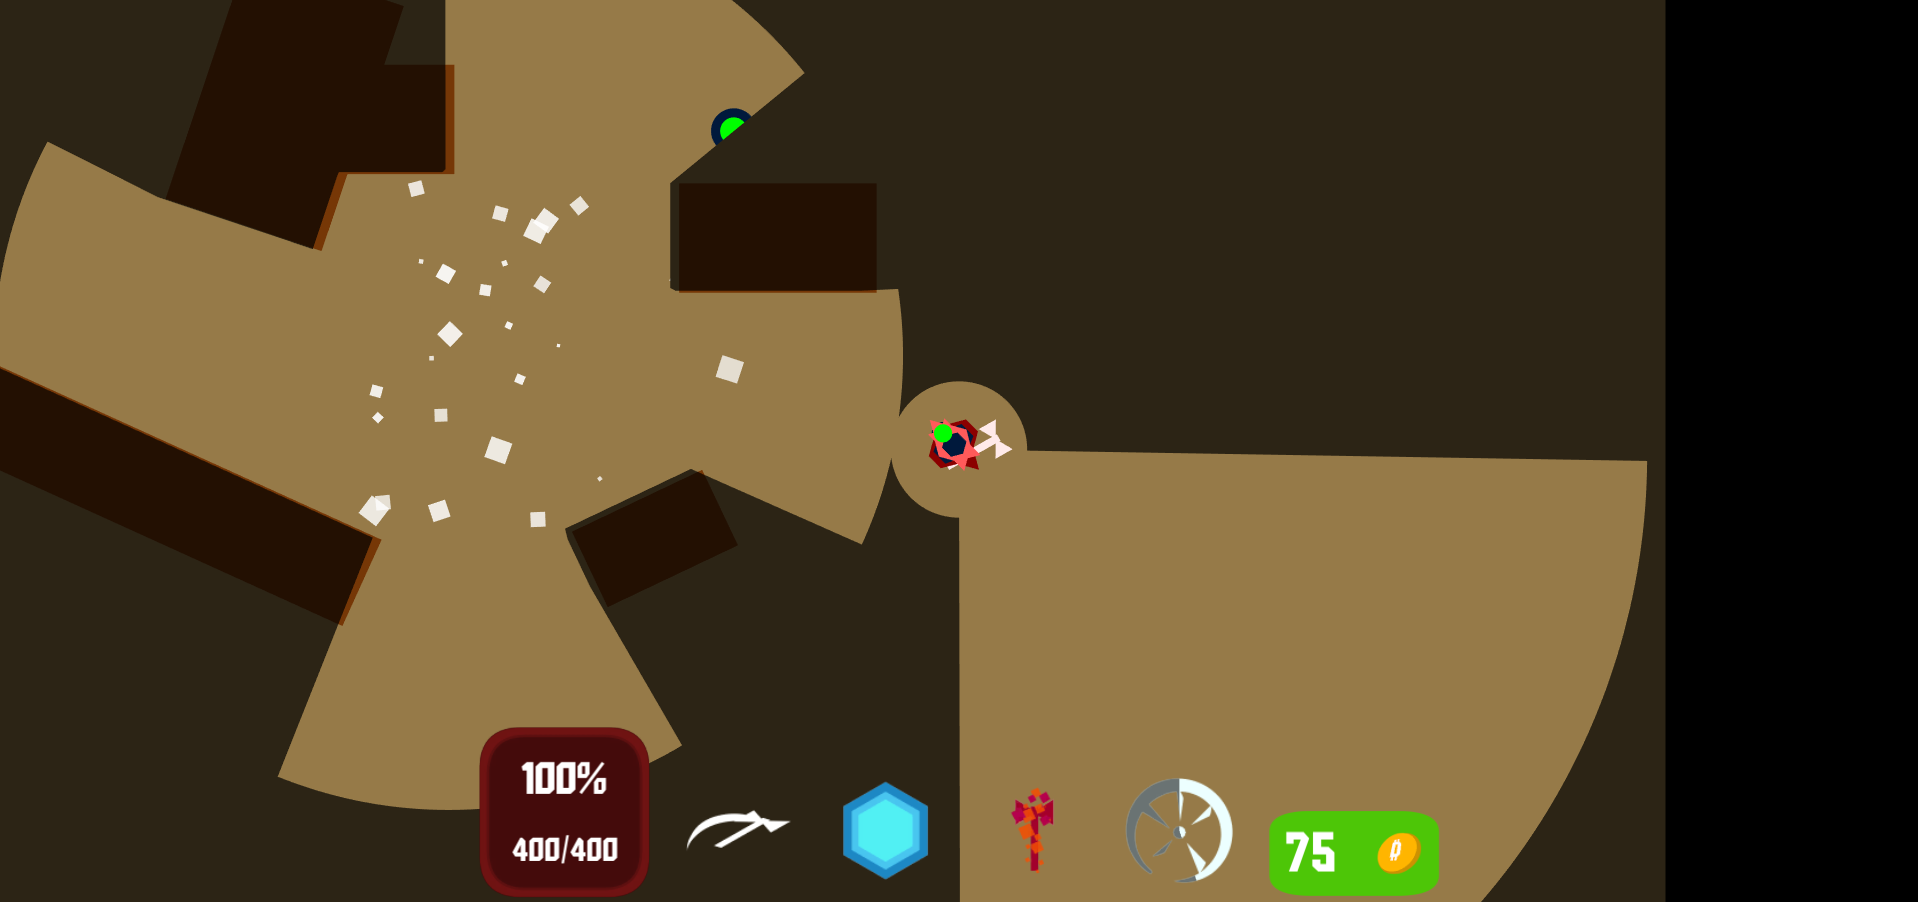
\includegraphics[width=.75\textwidth]{images/stunGrenade}
  \caption[Screenshot of the brawler kit's stun grenade]{A screenshot from the game showcasing the additional vision range granted from an exploded stun grenade}
  \label{fig:brawlerStunGrenade}
\end{figure}

The final ability makes the player throw a stun grenade that explodes after a short while, providing temporary vision for all players(see Figure~\ref{fig:brawlerStunGrenade}) and applying a stun modifier to anyone looking towards the explosion center. The grenade itself is a SpawnableObject and controls the application of modifiers, the temporary vision and any visual elements related to the grenade. The player on the other hand has a simple script that handles the spawning of the grenade. The grenade enables a large sphere collider on explosion which checks for any players within its range. A raycast is then used in conjunction with a dot product to check for players looking towards the center of the explosion. Players with obstacles between themselves and the explosion center will not get stunned as the raycast check will end up failing. 

\subsection{Marksman Kit}
\subsection{Sniper Kit}
\subsection{Tank Kit}

\subsection{Trapper Kit}
The Trapper Kit is a utility docking kit that focuses on using its three traps to provide various types of crowd control as well as being adequately capable of fighting enemies in close to mid range using the kit's flamethrower.  

The first ability in the kit is the flamethrower, a self applied modifier that activates a large sphere collider that checks for objects that it can burn. One of the limitations of working with Unity3D rather than Unity2D is that we don't have access to polygon colliders. Using polygon colliders would have made it possible to create a cone collider for this ability. We are instead using a large sphere collider for the flamethrower although its shape is not necessarily as fitting.
The collision callback checks for any enemy players and applies a burn modifier to these. It also checks for game objects with the IElement interface and applies a fire element to any such objects if found. This means that abilities from other kits that support elemental modifiers can be buffed by the flamethrower.

The three other abilities use traps deriving from a base Trap class. A shared TrapSpawner script is used to spawn each of the three traps by providing it with different prefabs per ability. 
The trap spawner script handles spawning its given trap prefab as well as updating the visuals of the docking kit to reflect that traps have been placed. Each trap has its own visual element on the docking kit that is modified to allow other players to know which traps the user currently has placed. Figure~\ref{fig:trapperKit} showcases these.
The trap spawner script contains a reference to the spawned trap while the spawned trap is provided with a reference back to its owner. This allows the trap to only stay visible for its owner as well as communicating back to its owner whenever it has been triggered. 

Acquiring the reference to the traps is handled by implementing the ISpawnableReferenceProvider interface. Only one trap of each type can be placed at a time so trying to replace a trap that already is placed destroys the old trap and places a new one at the player's current position.  

\begin{figure}[tbph]  %t top, b bottom, p page | you can also use h to try to get the figure to appear at the current location
  \centering
  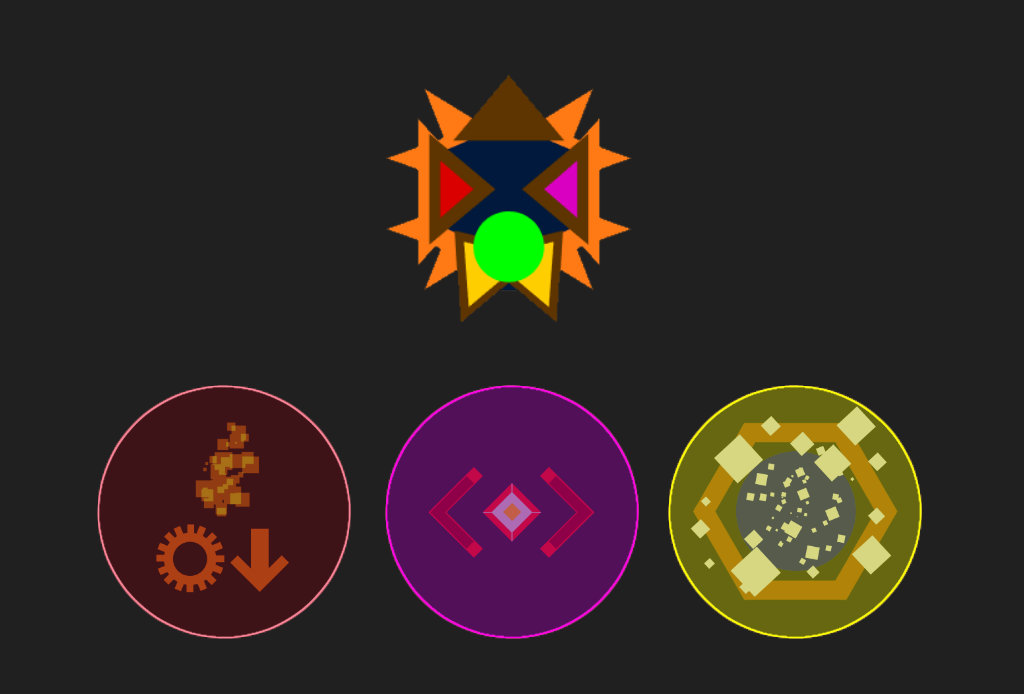
\includegraphics[width=.75\textwidth]{images/TrapperKitWithTraps}
  \caption[The trapper kit with its three traps]{The trapper kit has three traps. Placing one trap fades the color of its associated visual element on the docking kit}
  \label{fig:trapperKit}
\end{figure}

The Trap base class handles generic functionality like changing the visual state of the trap to invisible for other players as well as playing animations whenever the trap is triggered. A virtual function is used to allow any children of the base class to provide custom behaviour as the trap is triggered. The base class also contains a list of players that triggered it to make sure that no modifiers are applied twice in the case that a player quickly moves in and out of the trap collider. 

The two first traps have fairly simple behaviour. Both have modifiers that they apply to the list of players who triggered the trap. The first applies a burn and slow modifier while the second applies a blind modifier. 

The third trap has more custom behaviour compared to the previous two. It pulls in any nearby enemy players after triggering and places a temporary wall around these players to "capture" them for a short duration. There are a lot of different visual elements like particle systems, animations, colliders and sprites that are enabled/disabled throughout the trap's lifecycle. 

Applying the force for pulling players into the trap is done using a TargetRpc function located in the main player script while a C\# coroutine is used to enable the walls after a short duration. More information on adding consistent force to both the server and clients can be found in section~\ref{sec:conForce}. 

\subsection{Support Kit}

\section{Shop Architecture}
\subsection{Visual Layout}
\begin{figure}[tbph]  %t top, b bottom, p page | you can also use h to try to get the figure to appear at the current location
  \centering
  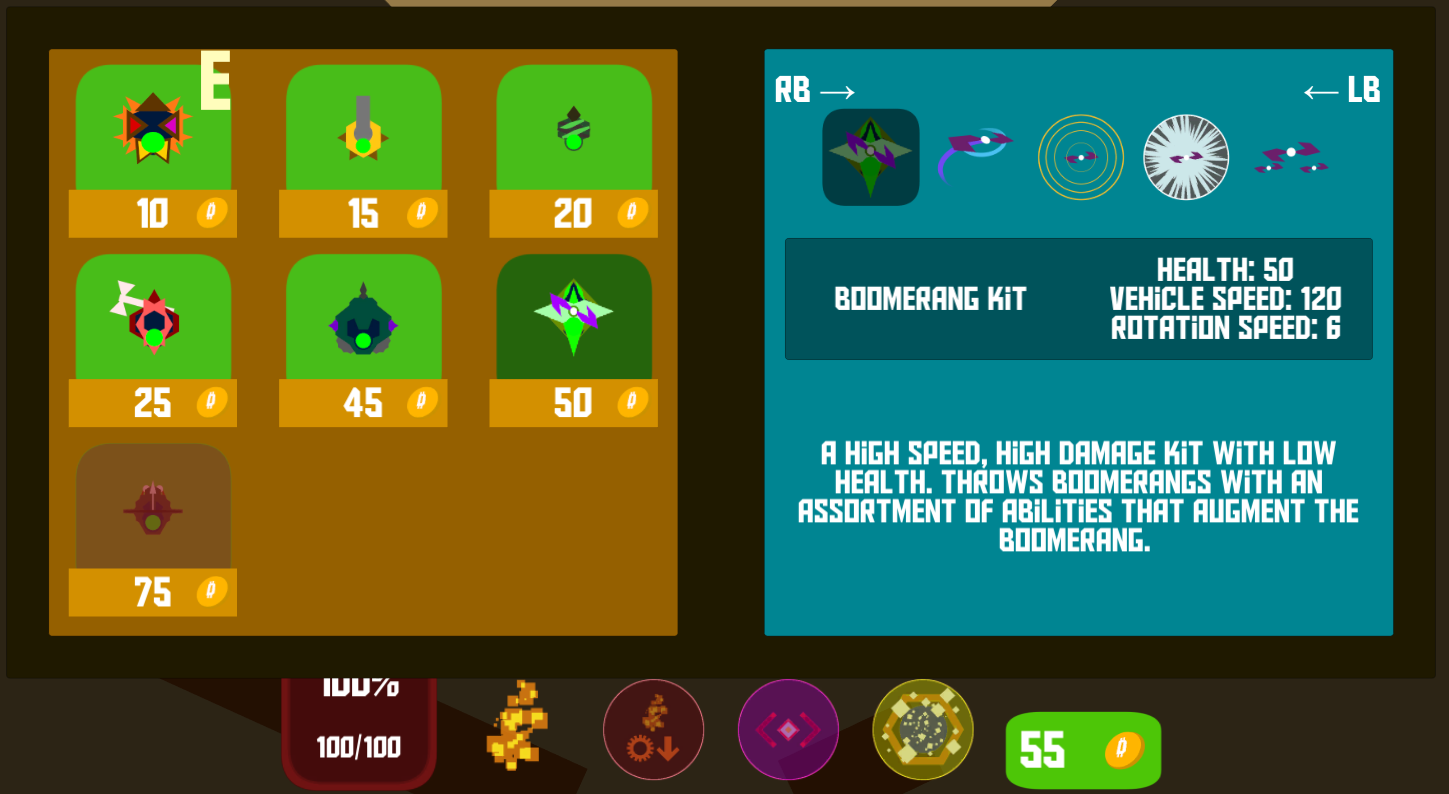
\includegraphics[width=.75\textwidth]{images/shopOverview}
  \caption[Screenshot showing off the in-game shop]{A screenshot showing off the in-game shop}
  \label{fig:shopOverview}
\end{figure}

The visual layout of the shop can be seen in Figure~\ref{fig:shopOverview}. The layout itself is split into two halves. 
The left half contains purchasable shop items while the right half contains individual information on the currently selected shop item. The currently equipped docking kit is signified by a "E" while any unpurchasable docking kits due to lack of currency are greyed out. 
The information display on the right side contains several text boxes that scripts can use to display arbitrary information about the shop item like names, descriptions and additional stats. Each docking kit contains information on the kit and its abilities which is split into five different "tabs". The information tabs for each item can be cycled through by pressing the left and right shoulder buttons on the controller as displayed on the top of the panel.

\subsection{Using scriptable objects for shop items}
Scriptable objects provide an easy to use interface for developers, especially if used as described in section*INSERT REFERENCE HERE*. It allows us to simply go the the correct resource folder, right click and choose "New shop item". We can then directly fill in any data related to the new shop item in the inspector as seen in Figure~\ref{fig:scriptableObjectInspectorShop}. 
The scriptable object for shop items contains several pieces of data:
\begin{itemize}
    \item The name of the docking kit.
    \item The sprite that is displayed in the left panel of the shop.
    \item The prefab for the related docking kit.
    \item The price of the docking kit
    \item An enum which we use as a ID to identify the docking kit.
    \item A list of structures containing description data. These structures include the sprites used for the tabs on the right panel of the shop, the name of the ability/kit and a description. 
\end{itemize}

The scriptable object itself does not contain any code and is used as a data container. The data within the scriptable objects are then loaded by the menu handler and attached to instantiated shop item instances. 

\begin{figure}[tbph]
  \centering
  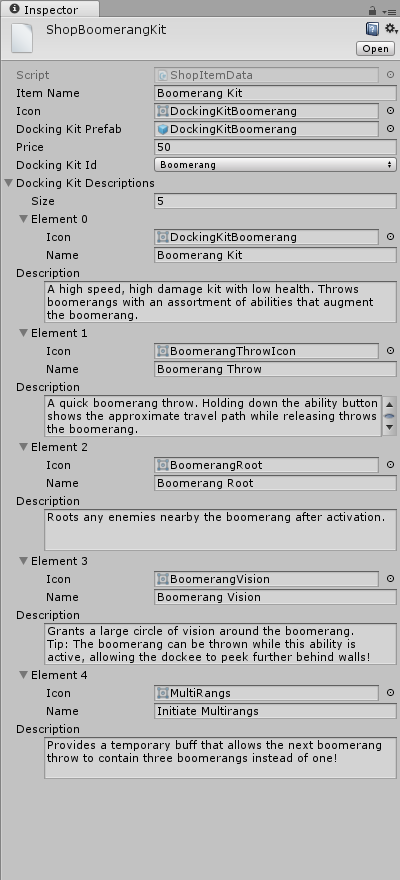
\includegraphics[width=.6\textwidth]{images/scriptableObjectInspector}
  \caption[Image of the Unity inspector showing scriptable objects from the shop]{An image of the Unity inspector that illustrates how one of the scriptable objects from the shop looks like}
  \label{fig:scriptableObjectInspectorShop}
\end{figure}

\subsection{How the shop is managed internally}
The shop architecture in Dockit League is split up into several components:
\begin{itemize}
    \item A script, IngameMenuHandler *APPENDIX LINK* manages the shop and any interaction with it.
    \item Scriptable Objects are used to contain data related to the individual shop items. 
    \item Each item instance in the shop contains the ShopItemInstance script *APPENDIX LINK* which stores a scriptable object and handles the data display for it. 
\end{itemize}

The IngameMenuHandler script starts by loading all scriptable objects within the project that contain item data. These scriptable objects are then placed in a list and sorted by price before the script starts instantiating ShopItemInstance's with a respective scriptable object. 
The script also handles input for scrolling through the information tabs of the currently selected shop item. This is handled by incrementing and decrementing a range limited integer which is used as a index to access the correct descriptions from the scriptable object. 

We use a prefab with uninitialised visual elements and a ShopItemInstance script to spawn in individual shop items. After being spawned, the instance is then initialised by passing a scriptable object over to it and updating all of its visual elements with the acquired data. The ShopItemInstance script also contains a callback for whenever it is pressed which displays a purchase verification prompt with a "yes" and "no" answer. Answering "yes" to the prompt tells IngameMenuHandler to complete the purchase and equips the new docking kit to the player.  

\section{Standard Game Flow}
